

Geomecânica é o estudo das deformações e tensões em solos e rochas, esse estudo se torna de extrema importância para a explotação de campos de petróleo de maneira segura e mais eficiente. De acordo com \citet{ResGeomec}, o estudos de tensões são importantes, pois:

\begin{itemize}
    \item Falhas em poços ocorrem por conta de tensões concentradas ao redor da circunferência dos poços.
    \item Falha geológicas vão deslizar dependendo das tensões e da sua resistência a fricção. 
    \item Depleções do reservatório causam mudanças nas tensões \textit{in-situ} que podem ser maléficas ou benéficas para a produção.
\end{itemize}

Além disso, deformações na rocha devido a produção causam subsidência do leito marinho que podem tanto causar problemas ambientais como danificar equipamentos de sub-superfície. Injeção demasiada de água  pode reativar falhas ou provocar fraturas na rocha capeadora fazendo com que aconteçam exsudações de óleo na superfície. Assim, fica claro que os estudos de geomecânica são importantes para uma melhor produção do campo, redução de custos de explotação e também para uma operação mais segura.  E para a realização desses estudos é importante a utilização de simulações geomecânicas capazes de representar a realidade a fim de evitar problemas no campo.

Os modelos geomecânicos, diferentemente dos modelos de fluxo de reservatório, estão interessados em fenômenos que ocorrem em regiões que são não reservatório como os exemplos de subsidência e tensões ao longo da trajetória do poço do parágrafo anterior. Assim, os modelos necessitam de um domínio de simulação maior que o das simulações de fluxo, contento regiões de \textit{overburden}, \textit{sideburden} e \textit{underburden}. A Figura \ref{fig:modelogeomec3d} mostra um corte de um grid de um modelo geomecânico em três dimensões, os elementos pintados de azul são relacionados ao reservatório. Pode-se ver que este corresponde a uma pequena parte do modelo, isso faz com que o número de elementos dos  modelos sejam grandes, tornando necessárias técnicas numéricas e de computação de alto desempenho com boa performance para que as simulações possam ser realizadas em tempo viável. 


\begin{figure}[!htbp]
\centering
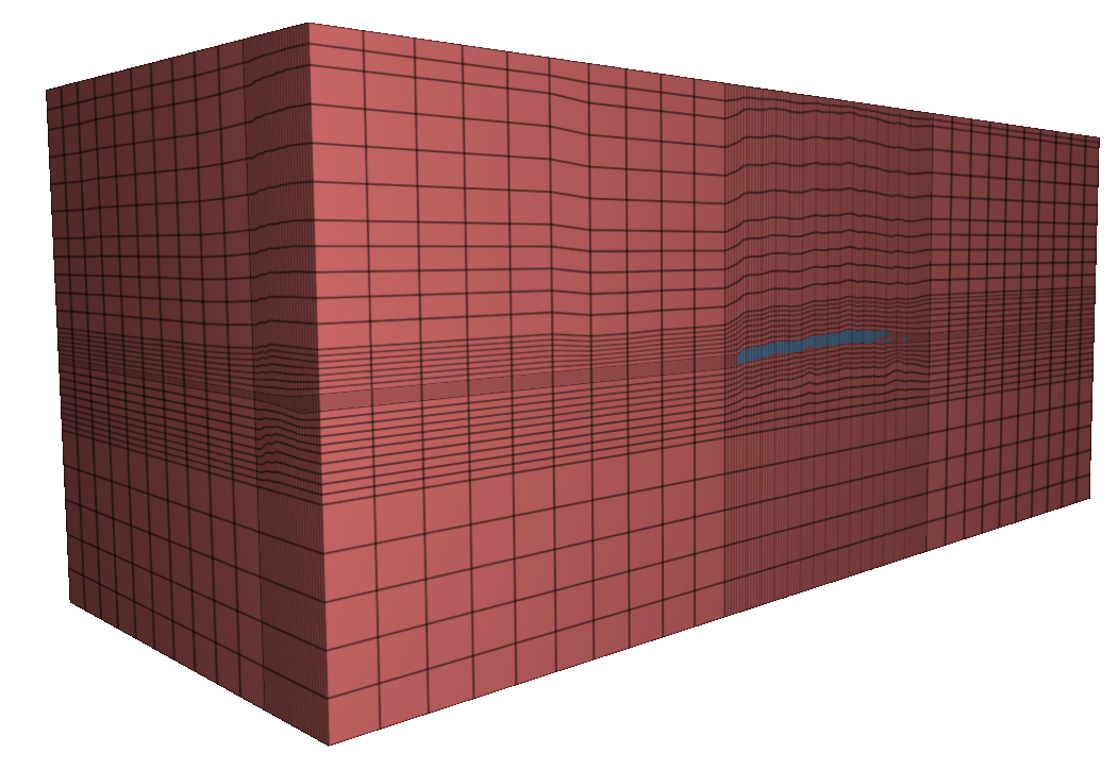
\includegraphics[width=10cm]{chap00/figs/Geresim(0054).png}
\caption{Corte vertical de modelo geomecânico 3D. Células em azul representam o reservatório.}
\label{fig:modelogeomec3d}
\end{figure}

Em geral, os simuladores gastam a maior parte do tempo resolvendo sistemas lineares e, portanto, melhorias realizadas nos solvers são bastante impactantes nos tempos das simulações. Tendo isso em vista, essa dissertação tem como intuito avaliar um pré-condicionador multiescala para reduzir o número de iterações de solver lineares de Krylov, em particular, para o Gradiente Conjugado e Bicgstab. Ela é organizada da seguinte forma: no Capítulo \ref{ch:modelagem} são apresentadas as equações que regem os fenômenos geomecânicos, no Capítulo \ref{ch:discretizacao} é apresentado a discretização realizada nas equações do capítulo anterior através do método dos elementos finitos chegando a um sistema linear, no Capítulo \ref{ch:sistemas} são apresentadas estrutura de dados para matrizes esparsas e métodos para solução de sistemas lineares, no Capítulo \ref{ch:multiescala} é apresentado o método multiescala e como ele pode ser utilizado como pré-condicionador para acelerar métodos iterativos de solução dos sistemas lineares, no Capítulo \ref{ch:implementacao} são apresentados detalhes da implementação realizada nesse trabalho e, finalmente, no Capítulo \ref{ch:resultados} são apresentados os experimentos numéricos, onde se destacam a comparação entre pré-condicionador aditivo e multiplicativo e comparação com o método multigrid. 


% Além disso, os efeitos geomecânicos também são importantes também tem influência no fluxo por conta de modificações no volume poroso e também na permeabilidade do modelo. Conforme mostrado em \citet{rolegeomechanics} as diferenças de produção podem ser consideráveis em uma simulação de fluxo em relação a uma simulação acoplada.


